\documentclass[authoryear,11pt]{elsarticle}

%This eliminates the `Preprint submitted to...' footer on the first page
\makeatletter
\def\ps@pprintTitle{%
 \let\@oddhead\@empty
 \let\@evenhead\@empty
 \def\@oddfoot{}%
 \let\@evenfoot\@oddfoot}
\makeatother

\usepackage{amssymb}
\usepackage{amsthm}
\usepackage{caption}
\usepackage{amsmath}
\usepackage{morefloats}
\usepackage{bbm}        %To allow \mathbb{1}

\usepackage{rotating}   %To turn tables sidewaystable
\usepackage{graphicx}
\usepackage{setspace}
\usepackage{hyperref}

%\onehalfspacing

%\setlength{\parindent}{0pt}

\usepackage[top=3.5cm,bottom=3.75cm,left=2.45cm,right=2.45cm]{geometry}% by courtesy of Mico

\begin{document}
\begin{frontmatter}
\title{MFE Economics\\Problem set 5}
\end{frontmatter}

%%%%%%%%%%%%%%%%%%%%%%%%%%%%%%%%%%%%%%%%%%%%%%%%%%%%%%%%%%%%%%%%%%%%%%%%%%%%%%%%%%%%%%%%%%%%%%%%%%%%%%%%%%%%%%%%%%%%%%%%%%%%%%%%%%%%%%%%%%%%%%%%%%%%%%%%
%%%%%%%%%%%%%%%%%%%%%%%%%%%%%%%%%%%%%%%%%%%%%%%%%%%%%%%%%%%%%%%%%%%%%%%%%%%%%%%%%%%%%%%%%%%%%%%%%%%%%%%%%%%%%%%%%%%%%%%%%%%%%%%%%%%%%%%%%%%%%%%%%%%%%%%%

\section{Technical: Gal\'i composite shock}
Although it is natural to look for equilibrium functions for the endogenous variables in terms of the fundamental shocks, such as
\begin{eqnarray*}
\pi_{t} 		&=& \psi_{\pi,a} a_{t} + \psi_{\pi,z} z_{t} + \psi_{\pi,v} v_{t} \\
\tilde{y}_{t} &=& \psi_{\tilde{y},a} a_{t} + \psi_{\tilde{y},z} z_{t} + \psi_{\tilde{y},v} v_{t}
\end{eqnarray*}
Gal\'i looks for expressions in terms of the `composite' shock, $u_{t}$ (in Ch. 3, P. 65 onward)
\begin{eqnarray*}
\pi_{t} 		&=& \psi_{\pi,u} u_{t} \\
\tilde{y}_{t} &=& \psi_{\tilde{y},u} u_{t} \\
u_{t}		&=& -\psi_{yn,a}\left( \phi_{y} + \sigma(1-\rho_{a}) \right)a_{t} + (1-\rho_{z})z_{t} - v_{t}
\end{eqnarray*}
He then makes the assumption that $u_{t}$ follows an AR(1) and then derives $\psi_{\pi,u}$ and $\psi_{\tilde{y},u}$ - i.e. he solves the model treating $u_{t}$ as the only state.

Without going into detail, this approach relies very heavily on the linearity of the model and an assumption that $u_{t}$ follows an AR(1) (which it isn't), rather than acknowledging that it is the sum of different AR(1) processes. Nevertheless, if one calculates the response to an innovation to $u_{t}$ then one can in fact use that response to derive the correct responses to innovations to $a_{t}$, $z_{t}$ and $v_{t}$.
\begin{itemize}
\item	What values of impulses to the various fundamental shocks (i.e. $\delta_{a}$, $\delta_{z}$ and $\delta_{v}$) will induce a unit impulse in $u_{t}$?
\item	What innovation simultaneously to $v_{t}$ will cancel out an innovation to $z_{t}$? Give some intuition and what is the implication for monetary policy (HINT: Compare a fundamental desire to save with a response to an additional incentive to save].
\end{itemize}

\subsection*{Answers}
We obtain the values simply through inverting the coefficients in the equation defining $u_{t}$\ldots
\begin{eqnarray*}
\delta_{a} &=& -\frac{1}{\psi_{yn,a}\left( \phi_{y} + \sigma(1-\rho_{a}) \right)} \\
\delta_{z} &=& \frac{1}{1-\rho_{z}} \\
\delta_{v} &=& -1
\end{eqnarray*}

To offset an innovation to $v_{t}$, $\delta_{v}$, the innovation to $z_{t}$ would need to be $\delta_{z} = \frac{\delta_{v}}{1-\rho_{z}}$

\section{First half technical - second half economic: DIS and NKPC}
The New Keynesian Phillips curve (NKPC) is given by
\begin{eqnarray*}
y_{t} &=& E_{t}[y_{t+1}] - \frac{1}{\sigma}(i_{t} - E_{t}[\pi_{t+1}] - \rho) + \frac{1}{\sigma}(1-\rho_{z})z_{t} \\
\pi_{t} &=& \beta E_{t}[ \pi_{t+1} ] + \kappa \tilde{y}_{t}
\end{eqnarray*}

\begin{itemize}
\item	Sketch a plot of the NKPC with $\tilde{y}_{t}$ on the horizontal axis and $\pi_{t}$ on the vertical axis.
\item	What is the slope?
\end{itemize}
Note that implicitly the location of the curve depends on assumed values for the structural parameters ($\beta$ and recall $\kappa$ is a function of various parameters) and expected inflation next period ($E_{t}[\pi_{t+1}]$).
\begin{itemize}
\item	What happens to the curve in the following situations? Give intuition.
	\begin{itemize}
	\item	Suppose something shifts $E_{t}[\tilde{y}_{t+2}]$ up, holding all else equal.
	\item	Suppose something shifts $E_{t}[\tilde{y}_{t+3}]$ up, holding all else equal. Compare to your previous answer.
	\item	What if $\theta$ increases, or $\varphi$?
	\end{itemize}
\item	Why is `holding all else equal' an unnatural assumption in this context?
\end{itemize}

\subsection*{Answers}
Turning to the NKPC, the right hand side of figure \ref{fig:dis_nkpc} shows that it is an upward sloping relations, with slope $\kappa$. Recall that $\kappa$ is defined as follows
\begin{eqnarray*}
\lambda 			&\equiv& 	\theta^{-1}(1-\theta)(1-\beta\theta)\Theta > 0 \\
\Theta 			&\equiv& 	\frac{1-\alpha}{1-\alpha + \alpha \varepsilon} \\
\kappa			&\equiv&	\lambda \left(\sigma + \frac{\varphi + \alpha}{1-\alpha}  \right)
\end{eqnarray*}

Now, what if $E_{t}[\tilde{y}_{t+2}]$ increases, holding all else equal? Note that $E_{t}[\tilde{y}_{t+2}]$ doesn't figure explicitly but recall that we can re-express the relation as
\[
\pi_{t} = \kappa \sum\limits_{k=0}^{\infty} \beta^{k} E_{t}[ \tilde{y}_{t+k} ]
\]
so we see that there will be a rightward shift in the curve, or perhaps it is more natural to think of it as an upward shift. Future output gap is expected to be higher and, thus, future marginal costs are expected to be higher, all else equal, so firms setting their prices today anticipate this (recall they are forward looking due to the fact the price they set today may prevail for several periods) and raise their prices more then they otherwise would have given the \emph{current} output gap, implying higher inflation (hence the `shift' upwards). The next part of the question is pretty much the same but the shift will be smaller for a given change in future expected output gap because it is weighted by $\kappa \beta^{3} < \kappa \beta^{2}$. Again, holding everything else equal is somewhat unnatural in this context, perhaps most obviously because any news today that the output gap will (in expectation) be higher in two (or three) periods' time will `likely' imply that expectations of the output gap will shift at other horizons too.

Regarding changes in parameters, as discussed in the previous homework, an increase in $\theta$ lowers $\lambda$ and thus flattens the slope of the curve. In contrast, increasing $\varphi$ steepens the Phillips curve.

\begin{figure}[!htb]
\center{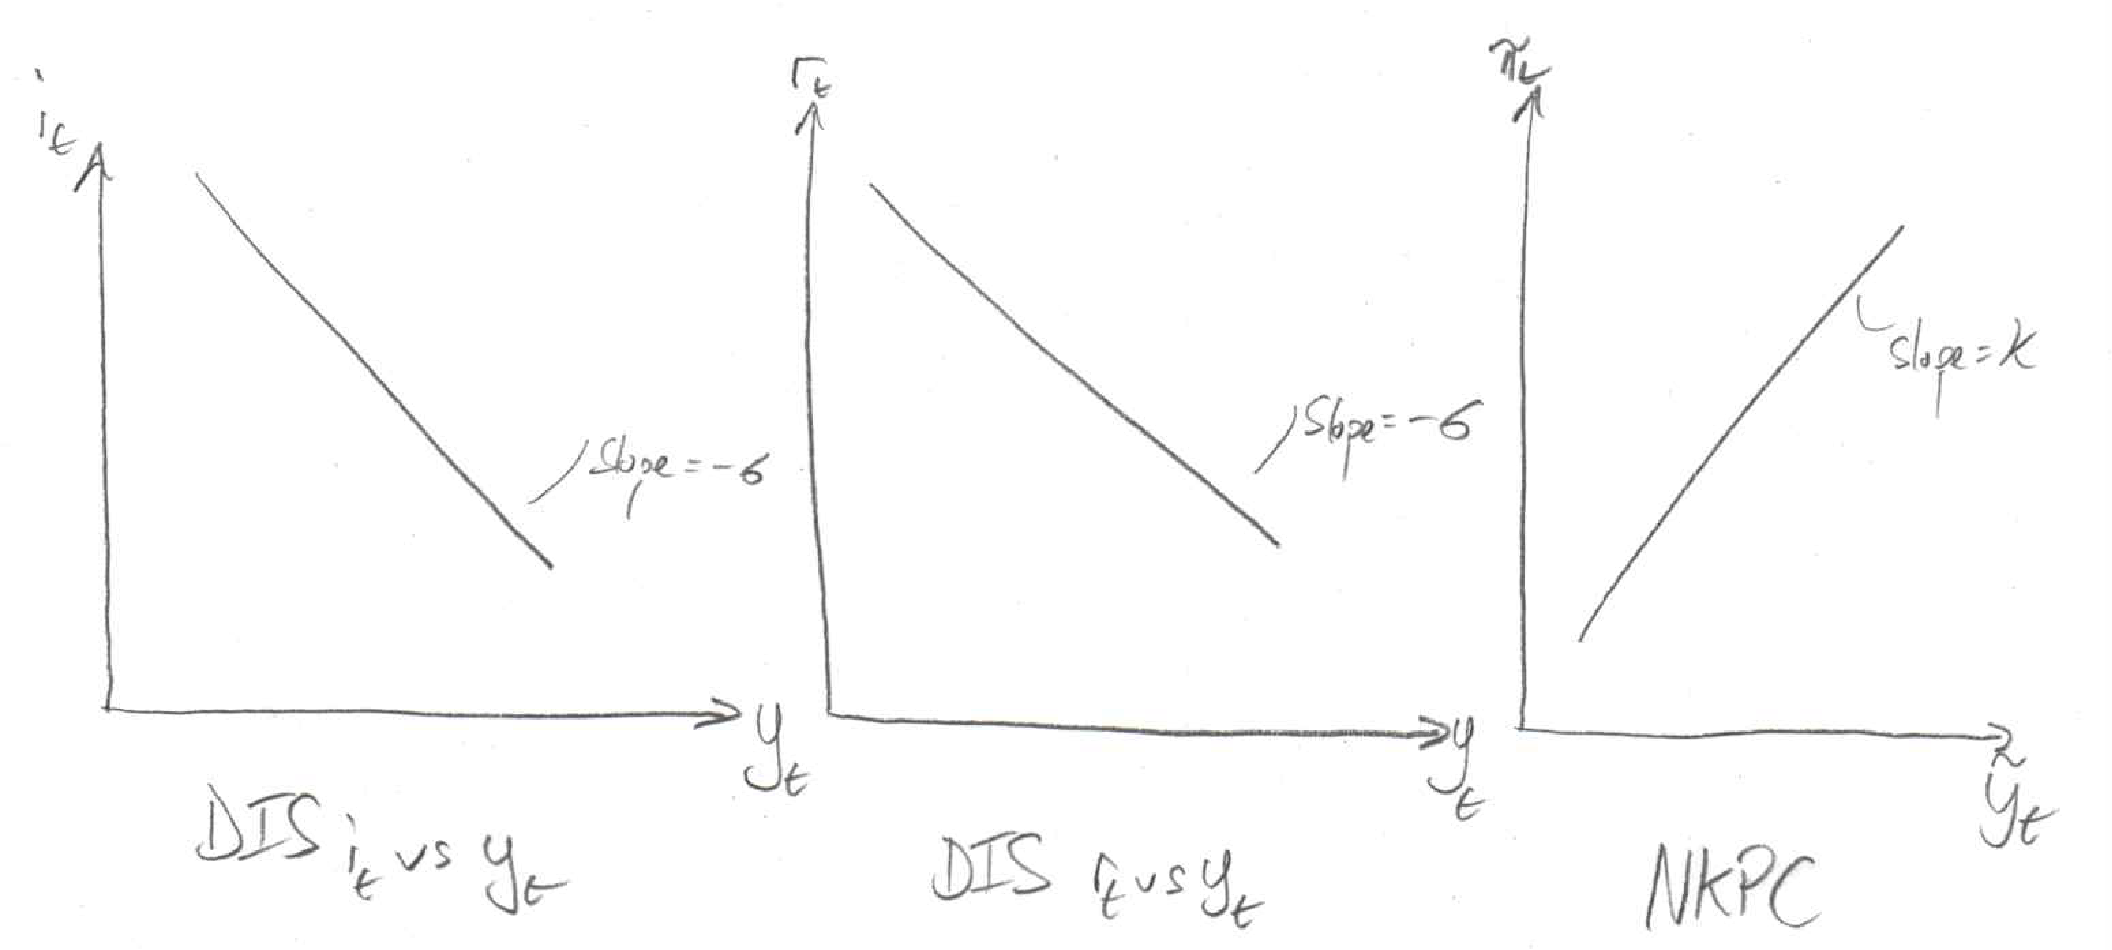
\includegraphics[width=1.0\textwidth]{dis_nkpc_figure.pdf}}
\caption{\label{fig:dis_nkpc} Sketch Dynamic IS and New Keynesian Phillips Curves}
\end{figure}

\section{Technical: Autoregressive processes}
[This is a continuation of the AR question in the previous problem set] In the models we consider we will often express the equilibrium values of endogenous variables as functions of $a_{t}$ (and other shocks). Suppose a variable $s_{t}$ is expressed
\[
s_{t} = \psi_{0} + \psi_{1} a_{t}
\]
\begin{itemize}
\item	What is $s_{t+1}$ in terms of $a_{t+1}$?
\item	What is $s_{t+1}$ in terms of $a_{t}$ and $\varepsilon_{a,t+1}$?
\item	What is the expected value of $s_{t+1}$ given information available in $t$ (i.e. given you know $a_{t}$)?
\item	What is the expected value of $\Delta s_{t+1} \equiv s_{t+1} - s_{t}$ given information available in $t$
\end{itemize}

\subsection*{Answers}
We have in terms of $a_{t+1}$ or in terms of $a_{t}$ and $\varepsilon_{t+1}$
\begin{eqnarray*}
s_{t+1} &=& \Psi_{0} + \Psi_{1} a_{t+1}	\\
s_{t+1} &=& \Psi_{0} + \rho \Psi_{1} a_{t} + \Psi_{1} \varepsilon_{t+1}
\end{eqnarray*}

The expected value of $s_{t+1}$ given $t$ information is
\[
E_{t}[s_{t+1}] = E_{t}[ \psi_{0} + \psi_{1} a_{t+1} ] = \psi_{0} + \psi_{1} E_{t}[ a_{t+1}] = \psi_{0} + \psi_{1} \rho a_{t}
\]

And the expected change in $s_{t+1}$ is
\[
E_{t}[ \Delta s_{t+1} ] = E_{t}[  \psi_{0} + \psi_{1} a_{t+1}  -  \psi_{0} - \psi_{1} a_{t} ] = \psi_{1} E_{t}[\Delta a_{t+1}] = \psi_{1} (\rho-1) a_{t}
\]

\section{Technical and a bit of intuition: Definitions of IRFs}
Our equilibrium implies variables, say $y_{t}$, can be expressed in terms of three shocks
\[
y_{t} = \psi_{y} + \psi_{y,a} a_{t} + \psi_{y,z} z_{t} + \psi_{y,v} v_{t}
\]

%In class, we defined the impulse response of $y_{t}$ to $a_{t}$ as the difference between the paths of $y_{t}$ under two different sequences of innovations. We called one, the `baseline' path and the other, the `shocked' path. The baseline path of the economy entails
\[
\varepsilon_{a,t}=\varepsilon_{z,t}=\varepsilon_{v,t}=0 \text{  }\forall t
\]
and the shocked path of the economy entails
\begin{eqnarray*}
\varepsilon_{a,1} &=& \delta_{a} \\
\varepsilon_{a,t} &=& 0 \text{  }\forall t>1 \\
\varepsilon_{z,t}=\varepsilon_{v,t}&=&0 \text{  }\forall t
\end{eqnarray*}
As shown in class this yields the impulse response function
\[
\Delta_{y,a}(t) = \psi_{y,a} \rho_a^{t-1} \delta_{a}
\]

\begin{itemize}
\item	What is the `impact effect' (i.e. effect in $t=1$ when the innovation hits)?
\item	Consider two sizes of impulse $\delta_{a}^{(B)} > \delta_{a}^{(S)} > 0$. Comment on the relationship between the impulse response to these two differently sized impulses - take their difference and their ratio. What does the ratio depend on (really, what does in \emph{not} depend on)? \emph{Hint: Try to distinguish magnitude from shape.}
\item	Consider two impulses, $\delta_{a}$ and $-\delta_{a}$. Comment on the relationship between the impulse response to these two differently signed impulses - take their ratio.
\item	In what way does the impulse response depend on the value of $a_{t}$ prevailing in the period before the impulse?
\item	Do the properties you derived in the previous part of this question seem `sensible'? Can you think of some simple examples/stories where the effect of an impulse might be dependent on the size/sign of the impulse and the state the economy is in on impact (in a more meaningful way than they do in our case)?
\end{itemize}

We defined an IRF by comparing two paths under a sequence of assumed future innovation realizations. Suppose \emph{instead} someone (very reasonably) might want to think of an impulse response as how his/her \textbf{expectations} of the future might change, given an impulse today. In this case we will calculate the difference in expectations after the impulse vs without the impulse, acknowledging that future innovations are random variables.\footnote{We continue to assume $\varepsilon_{z,1}=\varepsilon_{v,1}=0$}
\begin{itemize}
\item	What is the impulse response under this new approach of defining it as the difference in expected values of $y_{t+j}$ conditional on $\varepsilon_{a,1}=\delta_{a}$ and conditional on $\varepsilon_{a,1}=0$? NOTE: For this part of the question, eliminate $z_{t}$ and $v_{t}$ from the analysis, just to simplify the algebra slightly.
\end{itemize}

\subsection*{Answers}
The impact effect in this case is $\psi_{y,a} \rho_a^0 \delta_{a} = \psi_{y,a} \delta_{a}$. Now, under the two differently sized innovations we have the difference between the IRFs as
\[
\psi_{y,a} \rho_{a}^{t-1} (\delta_{a}^{(B)} - \delta_{a}^{(S)})
\]
and the ratio
\[
\frac{\delta_{a}^{(B)}}{\delta_{a}^{(S)}}
\]
The point here is that, obviously, the IRFs depend \emph{in some sense} on the size of the initial impulse (bigger impulse means bigger response), but it is not a particularly `interesting' dependence. In particular, the shape of the impulse response is effectively pinned down by the persistence parameter, $\rho_{a}$ so that the two responses are scaled versions of eachother with, as the ratio shows, the scaling being determined by the relative size of the impulse. Similarly, if we compare impulses under a positive and negative impulse we find that the ratio is $-1$. Again, this is not a very meaningful difference as the responses are essentially the same but flipped, as we would expect. Also note that none of these responses make any reference to the value of $a_{0}$ - the technology prevailing prior to the innovation.

Thus, if you tell me one IRF in a model such as ours, you've essentially told me all IRFs (for the same shock). This means that when working with models such as this, it isn't that vital to specify the size or type of shock when plotting pictures of IRFs, as long as one is consistent. However, there is the convention that one picks meaningful sizes so the reader doesn't have to do the (easy but tedious) math to get a sense of what the model is saying. For example, people often pick the size of the innovation to be equal to a single standard deviation (in this case that would be $\sigma_{a}$) with the understanding that is the size of a `typical' shock. Alternatively, one might scale the innovation size so that a given variable has an interpretable movement on impact (such as picking a monetary policy shock to induce a $25$ basis point change in $i_{t}$ - which might be though to be a relevant size of surprise, given Fed behavior).

Beware, however. This is an extremely special property of the linear models we have been dealing with (or at least they are linear after all our first order approximations). Nonlinear models (and the real world) will not exhibit this property - at least qualitatively (it is an empirical question how important nonlinearities are). Generally, we believe that a massive shock to, say, monetary policy, may have a different effect even beyond scaling and there is a lot of work discussing whether cuts in interest rates have the same effect as increases. Also, perhaps reflecting worse scope to borrow - and various other malfunctioning aspects of the economy - there is sometimes the belief that fiscal stimulus can be more effective when the `state' of the economy is a recession - suggesting that the impact of a fiscal shock might be different, depending on what the economy looks like when it hits. Linear models do not allow this and traditional IRF analysis of the type we have been using is inadequate to model this.\footnote{If you are interested see \href{https://www.richmondfed.org/-/media/richmondfedorg/publications/research/economic_brief/2017/pdf/eb_17-03.pdf}{here}, \href{https://www.sciencedirect.com/science/article/pii/0304407695017534}{here} and \href{https://www.aeaweb.org/articles?id=10.1257/0002828053828518}{here}.}

Another aspect of our assumption of linearity (and symmetric shocks, in fact) that is very special is that the redefined IRF (in terms of differences in expectations) gives the same answer as our originally defined IRF. This again reflects linearity of the model and the linearity of the expectations operator, as shown below\ldots

First, follow the (small) simplification suggested in the question
\[
y_{t} = \psi_{y} + \psi_{y,a} a_{t}
\]
and (recalling problem set 2) note that
\[
a_{t} = \sum\limits_{j=0}^{t-1} \rho_{a}^{j} \varepsilon_{a,t-j} + \rho^{t} a_{0}
\]
The innovation hits in $t=1$ ($\varepsilon_{a,1}=\delta_{a}$) so we are looking for the difference in expectations of $y_{t}$ conditional on $t=1$ information where in the baseline case, part of that information is $\varepsilon_{a,1}=0$ and in the shocked case, part of that information is $\varepsilon_{a,1}=\delta_{a}$. Thus we calculate
\begin{eqnarray*}
E_{1} [ y_{t} | \varepsilon_{a,1}=0 ] &=& E_{1} [ \psi_{y} + \psi_{y,a} a_{t} | \varepsilon_{a,1}=0 ] \\
&=& \psi_{y} + \psi_{y,a} E_{1} [  a_{t} | \varepsilon_{a,1}=0 ] \\
&=& \psi_{y} + \psi_{y,a} E_{1} \left[\rho_{a}^{t-1} \varepsilon_{a,1} + \sum\limits_{j=0}^{t-2} \rho_{a}^{j} \varepsilon_{a,t-j} + \rho^{t} a_{0} | \varepsilon_{a,1}=0 \right] \\
&=& \psi_{y} + \psi_{y,a} \rho^{t} a_{0}
\end{eqnarray*}
and we also calculate
\begin{eqnarray*}
E_{1} [ y_{t} | \varepsilon_{a,1}=\delta_{a} ] &=& E_{1} [ \psi_{y} + \psi_{y,a} a_{t} | \varepsilon_{a,1}=\delta_{a} ] \\
&=& \psi_{y} + \psi_{y,a} E_{1} [  a_{t} | \varepsilon_{a,1}=\delta_{a} ] \\
&=& \psi_{y} + \psi_{y,a} E_{1} \left[\rho_{a}^{t-1} \varepsilon_{a,1} + \sum\limits_{j=0}^{t-2} \rho_{a}^{j} \varepsilon_{a,t-j} + \rho^{t} a_{0} | \varepsilon_{a,1}=\delta_{a} \right] \\
&=& \psi_{y} + \psi_{y,a} (\rho^{t} a_{0} + \rho_{a}^{t-1} \delta_{a})
\end{eqnarray*}
Taking the difference of these we obtain $\psi_{y,a} \rho_{a}^{t-1} \delta_{a}$ which is the same as under our previous definition.

\section{Economic awareness}
\begin{itemize}
\item	In a couple of paragraphs, explain the role of IRF analysis in assessing the effect of monetary policy on the economy. What is the consensus view? [HINT: See Walsh and Gali first chapters, some of the Ramey paper and if you can, early parts of Christiano, Eichenbaum and Evans]
\item	Explain how the New Keynesian Phillips curve relates to the original Phillips curve and expectations augmented Phillips curves. You should refer to the evolving attitude towards the existence of a tradeoff between inflation and output. [You will need to do some simple online research for this - keep your answers to a page max.] 
\item	In one paragraph, discuss the current debate about the flattening of the Phillips curve - extra points if you look up AOC's exchange with Jerome Powell.\footnote{There are no extra points.} [HARDER] In an even shorter paragraph - explain what a flat Phillips curve implies for the impact of a monetary policy shock on inflation.
\end{itemize}

\subsection*{Answers}
Answers to follow\ldots

\end{document}

